这系列献给学过线代,算过矩阵,尚未开悟的同学。
\section{重修线性代数1——历史}
\subsection{前言}
有个网友发私信给我,问能不能写篇线性代数的文章。我有点为难,在科学网写科普,面
向也是研究生和教师。线性代数是理工科大学生的基础课,有中学基础,就不难学,写了
怕没人看。他说,许多朋友和他都学过线性代数,考试也得A,只是学后仍然是一脑子浆
糊,如有文章梳理一下,相信很多读者会受益。我上网查一下,果然有评论说,这课观念
台阶起的太高,猛然从中学的经验数学进入抽象世界,很多人转不过来,大多数人是在学
习理论力学、统计分析、信号处理、控制理论或计算方法时,才领会一部分的。科学发展
至今,线性代数已是科学和工程不可或缺的基础了,在MATLAB等软件上计算和显示,如同
昨日之用计算器。它也是机器学习的基础。对于线性代数的应用,熟练的计算和证明已不
是关键,重要的是掌握概念,明白内涵,能否想象。而对这点稍微说些个人体会的,都被
网上群众赞为醍醐灌顶。好吧,既然这么有用,我就给还没有开悟的朋友充一回大神。

这个系列与“重修微积分”系列类似,面向已经学过线性代数,觉得做题考试读文章还行,
学过套路,但还没变成武功的人。希望通过这系列文章,能形成对线性世界的直观认知,
不仅对懵懂者和初学者有用,对玩矩阵还算溜的人也有帮助。

许多人以为数学很枯燥,需要毅力来学习。这是未见美景者言。枯燥是因为不能想象,死
记硬背才需要毅力。学习数学有点与物理一样,都要在脑中“看到”内容的图像,只是物理
用实验证明这想象中的世界是真实的,数学是用形式逻辑证明它是对的,经过了求证的跋
涉,最后在心中留下的,要有永久记忆住的画面。如果你对数学内容所知还只是公式推导,
那还只是在途中,没见到山后的风景,自然觉得郁闷。

线性代数理论主要是在20世纪发展的。对相关的内容,人们早先的兴趣在于解线性方程组,
莱布尼茨在17世纪用过行列式,18世纪有了用行列式求解的克莱姆法则,及直接求解的高
斯消元法。到了19世纪人们引进矩阵的概念和运算,意识到它与行列式的关系。这些都还
像是牛顿前的力学,散布着先哲们计算技巧和总结出规律的智慧珍珠,还未从抽象的高度
来统合成一种理论。20世纪初,数学走向严谨形式推理的公理化系统。作为抽象理论的线
性代数才逐渐成形,研究应用数学的和物理的人愕然发现,克莱姆法则也可以用在微分几
何,解方程的特殊函数不过是线性空间的基向量,量子力学中的力学变量可以用矩阵或算
符表示。这些不同的高深知识,其实只是一种简单抽象的知识在具体对象上的表现,我们
可以站在高处来俯视。到了现在,线性代数已是纯数学和应用数学的核心基础,放宽约定
深入挖掘则有抽象代数,加上拓扑约束走向无穷则有泛函分析,泛化成算子理论让解微分
方程与代数方程趋向统一,在计算机程序中有了它,向量和矩阵如同数量一样的方便表达
使用。而这种表达在物理、控制、计算、统计、信息科学和工程应用上,已经是在职必须
通晓的工具,以致于瑞典数学家Lars Garding说:“现在不熟悉线性代数的概念,以这样
的基础想去学自然科学,就和文盲差不多。”

线性代数在中国普及到工科要晚一些。 现在大约已是理工科的必修课,在 50 年前我上大学时还不是。所以教你们课的老师,也许还未能将其精髓传授。上大一时,我在图书馆翻看吉林大学王湘浩谢邦杰编的《高等代数》,教理论力学的老师路过,翻了一下书页,说你学这个没什么用。没用?可我还是觉得有趣,花了几星期读完,有中学数学基础看懂内容,
倒没什么难度,只是对书中的前言,“学习这门课,必须学会从空间和矩阵的不同角度来
看问题”,这段话还不大理解。这让我在学习中反复捉摸这意思,直到后来学了更多数学
时,才算彻底明白。领会这观念让我受益匪浅。这么说吧,这是数学抽象的门槛,过了这
一关,数学就能编织成图案印在脑中,多年不用还能凭印象说出内容。

数学从小学、中学到大学三个阶段,分别是观念改变的三个门槛。小学数学的核心是数的
四则运算,如果2件50元,3件100元,哪个更便宜还转不过来,那还停留在用手指计数的
阶段,甭学理工科了,玩别的更合适。中学基本是几何想象、掌握函数的概念、代数推理
和套公式应用,学好就能对付传统职业的需要。如今开始,这已不敷科技职业的应用了,
在计算机成为手头必备的计算工具,矩阵和向量的概念将是常识,它们把算术中养成的逐
个计算,变成适应于机器的批量处理。学习微积分和线性代数,过的是两个不同的门槛。
一个是理解无穷和收敛的概念,让你用逻辑来推测无法经验的无穷世界。另一个是数学抽
象的把握,能把数的一元对应关系推广到多元乃至各种数学实体,依照需要,能对同一对
象用不同的数学抽象来概括,又能把不同的数学处理归纳成是一样的,用统一的数学方法
来处理。真正领悟这一点,你就上了一个台阶,进到更深数学领域才懂欣赏。数学是用基
础知识层层堆高的学问,前面的基础没学好,即使靠死记硬背考试过了关,想象的大厦叠
的也是歪楼,再叠就倒了。所以数学差的人,未必不聪明,只是以前学夹生了,没及早纠
正。

\subsection{为什么学“线性代数”?}
人们最初的抽象起于计数时的数量,这是一维的标量,最简单有用的计算是相加和比例,
几千年的实践让它有了最直观的想象和应用。平面几何让想象进入二维,物理构造了三维
空间的真实。线性代数让你进一步理解n维乃至无穷维中这种相加和比例的运用。

算术是标量的计算,也就是对具体的实(复)数做加减乘除的算法,这单个变量和计算结果
的关系可以写成一元的函数。如有多个变量就写成多元函数,有多个结果就写成一组函数
。但从另一个角度来看,这多元变量值是一组数,这多个结果也是一组数,一组数也可以
打包看作是一个数学的实体,叫“向量”,相同长度的数组在相加和比例运算中,仍然是同
长度的数组,这封闭的群体叫做一个空间。空间中的成员看做一个点。未知的多元变量,
则是向量空间中变动的点,一组多元函数是定义域向量空间中的点,与函数组值向量空间
中点的对应,或称为映射。向量把一元的函数关系类比地推广到一组多元函数乃至无穷组
无穷多元函数,或表示为空间的映射,写成与单变量函数的同样形式,或在抽象空间上的
统一形式。这种简单清晰的表达,在理论和计算工具的应用上都极为方便。人们经过百年
时间,终于习惯了这一点,现在成为科学和工程的公共基础。

当然,仅仅这样的改写,除了表达方便、联想直观以外,并没有带来更丰富的内容。线性
代数类似于算术,关注最基本的相加和比例的运算,这样的关系称为线性。因为向量空间
中的元素对线性计算封闭,所以向量空间在数学上称为“线性空间”。当多元的变量和计算
结果表示为向量形式时,其线性关系的映射称为线性算子;它们表达为数组的形式时,它
们间的线性关系则可以表示为一个矩阵。这个线性的映射就是矩阵与向量的乘法运算。任
何有限维数的向量都可以表示成一个有限长度的数组,有限维向量空间上的线性映射都对
应着一个矩阵。线性代数研究怎么玩得转它们。

线性意味着一种容易计算,可以简单向前推测的系统。重要的是,这样的系统可以用数乘
来比例放大,用叠加原理来综合。科学研究经常把一个系统分解成子系统,分别研究它们,
然后综合它们的结果从而了解整体。例如力学中计算形变和运动用力的叠加,电路上电流
电压的叠加,力学声学光学中波的叠加,量子计算波函数的叠加,数理方程用函数族解的
叠加。科学研究从牛顿前的零敲碎打,到现在的分解综合是基于叠加原理。而叠加原理能
行得通,系统必须是线性的。

在中学,代数是“懒人的算术”,把需要技巧的算术变成照章办事。把算术题中已知数未知
数各自写成符号,按照算术中总结出的等价规则,来导出它们间的关系式。这样要计算同
一类的算术问题,就不需要按类型运用技巧了,通过机械的规则搬弄符号,约简成单一未
知数在左边已知数在右边的等式,代入计算就能得出答案。这是古希腊丢番图发明的一种
抽象方法,能够统一处理同一类的数学问题。在这种抽象下,对方法的研究形成理论,得
到的结果叫做公式。现代数学中的代数结构,是进一步地抽象,抽象的对象不是现实世界
的事物,而是数学中的概念和工具。研究抽象集合中一种或多种封闭的运算结构,如群、
环、域、格等,其中二元运算形成的抽象系统叫代数系统。总之,它代表作抽象的形式运
算观念。

线性代数就是从理论高度用抽象的方法,研究这类可叠加的系统,从线性空间映射的高度
看待它们中的运算,了解这些运算变换的结构。科学研究上凡是用到数学涉及计算,有着
漂亮定性和定量结果的,基本上是把它描写成线性系统,或者以此来逼近。所以它成为现
代科学和工程的公共基础。

\subsection{向量表示已是计算机数据表示的基础}

几个世纪前的数学家,曾经花费大量的精力来研究代数方程的解,期望后人只要学习他们
的成果,沿着开辟好的路径,按图索骥地前行。计算机时代,却把前人研究好的算法,打
包成为同一个程序,后人不需要了解蹊径,只要把数据也打包成统一的形式,就可以统一
处理。让我们先体验一下向量作为一个数组,在计算工具中的应用。
\kaishu
向量a是一组数,把它看成多项式的系数,它可以表达一个多项式或者代数方程。代数方
程所有的根x也是一个向量,方程的解可以看作以这向量作为变量的一个函数$ x=roots(a) $,
将任何代数方程表示成系数的向量,就可以代入这函数来求解。比如说解五次方程$ x^5-5x-2=0  $ 
,它没有根式解,但可以计算近似的数值解。\\
\\
\songti
\begin{center}% 令表格居中
\begin{tabular}{|p{150 pt}|p{150 pt}|}
\hline
\makecell[c]{在MATLAB或Octave\\
	指令窗口中打入:\\
Octave:1$ > $  a=[1,0,0,0,-5,-2];\\
Octave:2$ > $  x=roots(a)\\
在窗口中马上就显示\\
出这方程的5个根的数值,\\
x= \\
1.58204 +  0.00000i\\
0.09597  + 1.51080i\\
0.09597  - 1.51080i\\
-1.37188  + 0.00000i\\
-0.40210  + 0.00000i\\}
&
\makecell[c]{再打入指令\\
Octave:3$ > $  plot(x,'r*')\\
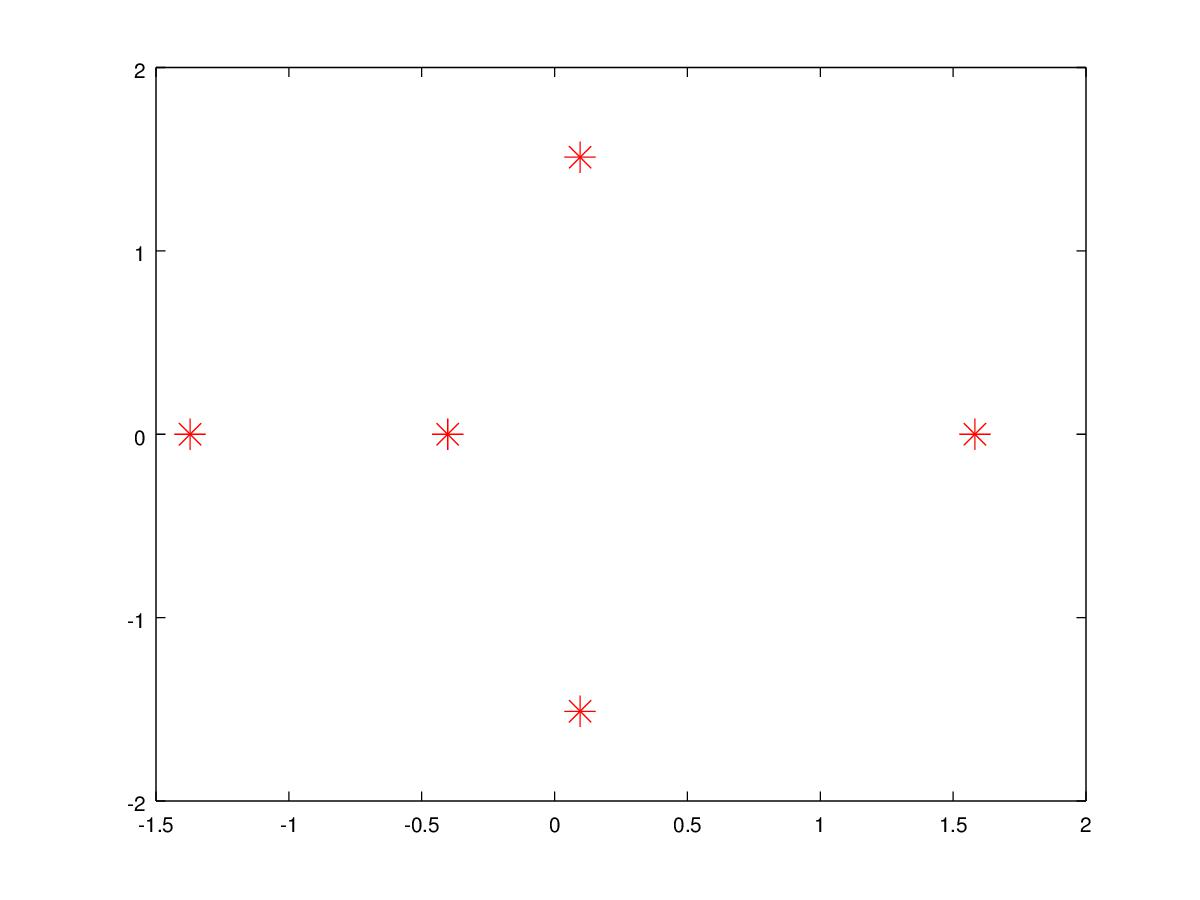
\includegraphics[width = .4\textwidth]{pic/163122zo5tmql5otmldxtf.jpg}\\
就画出这5个根在复平面的位置。}
\\
\hline
\end{tabular}
\end{center}



\kaishu
应用向量的表达,在今日可以很方便地与计算机互动来完成科研和工程中的计算和图像显
示工作。

\songti
\par
我们将从线性方程组、矩阵和线性空间,不同的角度,建立起它们的联系,让你从直观想
象中了解线性代数的内容。
